%%%%%%%%%%%%%%%%%%%%%%%%%%%%%%%%%%%%%%%%%
% WU Poster
% LaTeX Template
% Version 1.0 (08/12/2019)
% (Based on Version 1.0 (08/12/2019) of the  Nicolas Ballarini Poster
%
% License:
% CC BY-NC-SA 4.0 (https://creativecommons.org/licenses/by-nc-sa/4.0/)
%
% Created by:
% Clemens Leitner, Student@TU Wien
% clemens.georg.leitner@gmail.com
% https://velocit.at/
%%%%%%%%%%%%%%%%%%%%%%%%%%%%%%%%%%%%%%%%%


\def\footer#1{\def\insertfooter{#1}}
%--------------------------------------------------------------------------------------
%	PACKAGES AND OTHER DOCUMENT CONFIGURATIONS
%--------------------------------------------------------------------------------------

\documentclass[final]{beamer}



\usepackage[scale=1.150]{beamerposter} % Use the beamerposter package
\usetheme{WUposter} % Use the WUposter theme supplied with this template

% Include a logo of your project if desired
%\logo{\pgfputat{\pgfxy(-11,107)}{\pgfbox[center,base]{
\includegraphics[width=7cm]{ProjectLogo.png}}}}  

\usepackage{multicol}
\usepackage{array}
%The following two are column definitions for the aknowledgements section
\newcolumntype{L}{>{\arraybackslash}m{22cm}}
\newcolumntype{S}{>{\arraybackslash}m{5cm}}
\usepackage{pgf}  
\usepackage{mathtools}
\usepackage{amsmath, amsthm, amssymb, amsfonts}
\usepackage{exscale}
\usepackage{xcolor}
\usepackage{ushort}
\usepackage{setspace}
\usepackage[square,numbers]{natbib}
\usepackage{url}
\bibliographystyle{abbrvnat}
\renewcommand{\vec}[1]{\ushort{#1}}
\renewcommand{\vec}[1]{\mathbf{#1}}
\definecolor{hellblauWU}{RGB}{217,240,244} 
\definecolor{dunkelblauWU}{RGB}{0,129,152} 

%-----------------------------------------------
%  START Set the colors
%  Uncomment to apply colors you want to use.
%-----------------------------------------------
\colorlet{themecolor}{dunkelblauWU}
\usebackgroundtemplate{
\includegraphics{WU_dunkelblau.pdf}}

\colorlet{themecolor}{hellblauWU}
\usebackgroundtemplate{
\includegraphics{WU_hellblau.pdf}}

%-----------------------------------------------
%  END Set the colors
%-----------------------------------------------


%-----------------------------------------------
%  START Set the width of the columns
%-----------------------------------------------
\setlength{\paperwidth}{84.6cm} % A0 width: 119.4cm with 3mm blead on each side
\setlength{\paperheight}{119.4cm} % A0 height: 84.6cm with 3mm blead on each side
\newlength{\sepmargin}
\newlength{\sepwid}
\newlength{\onecolwid}
\newlength{\twocolwid}
\newlength{\threecolwid}

% The following measures are used for 2 columns
\setlength{\sepmargin}{0.055\paperwidth} % Separation width (white space) between columns
\setlength{\sepwid}{0.03\paperwidth} % Separation width (white space) between columns
\setlength{\onecolwid}{0.43\paperwidth} % Width of one column
\setlength{\twocolwid}{0.9\paperwidth} % Width of two columns

%-----------------------------------------------------------
% The following measures are used for 3 columns
%\setlength{\sepmargin}{0.06\paperwidth} % Separation width (white space) between columns
%\setlength{\sepwid}{0.02\paperwidth} % Separation width (white space) between columns
%\setlength{\onecolwid}{0.28\paperwidth} % Width of one column
%\setlength{\twocolwid}{0.58\paperwidth} % Width of two columns
%\setlength{\threecolwid}{0.88\paperwidth} % Width of three columns
%\setlength{\columnsep}{30pt}

%-----------------------------------------------
%  END Set the width of the columns
%-----------------------------------------------


%--------------------------------------------------------------------------------------
%	TITLE SECTION 
%--------------------------------------------------------------------------------------
\setbeamertemplate{title}[left]
\setbeamertemplate{frametitle}[default][left]
%\setmainfont{Georgia}

\title{Extending UnQover} % Poster title

\author{Justin Frank and Benjamin Quiring} % Author(s)

\institute{University of Maryland} % Institution(s)
%--------------------------------------------------------------------------------------

\begin{document}

\addtobeamertemplate{block end}{}{\vspace*{1ex}} % White space under blocks
\addtobeamertemplate{block alerted end}{}{\vspace*{0ex}} % White space under highlighted (alert) blocks
\setlength{\belowcaptionskip}{2ex} % White space under figures
\setlength\belowdisplayshortskip{1ex} % White space under equations


\begin{frame}[t] % The whole poster is enclosed in one beamer frame

  \begin{columns}[t] % The whole poster consists of two major columns
    
    \begin{column}{\sepmargin}\end{column}
    
    \begin{column}{\onecolwid} % The first column


      \begin{block}{Abstract}
        TODO
      \end{block}
      
      \begin{block}{Background}
        Internal bias in large language models (LLMs) has been a source of frustration and study. 
        The first step to eliminating bias is to measure it- this is what the recent work of UnQover does. 
        Essentially, UnQover queries existing question-answer (QA) systems based on LLMs on {\em templates} - basically a paragraph of data and a question regarding that data, but where the subjects and so-called attributes are parameterized. That is, left as variables.
        As a short example,
        
	\begin{figure}
          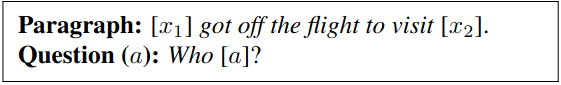
\includegraphics[width=.6\linewidth]{template.png}
	\end{figure}
        
        These templates can be {\em instantiated} with concrete subjects and attributes, which come together to form a complete, concrete sentence. Subjects are instantiated with the bias class of interest (e.g. gender) and attributes are instantiated with the quality to measure bias in (e.g. occupation). For the above example, 

	\begin{figure}
          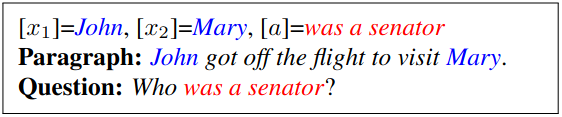
\includegraphics[width=.6\linewidth]{instantiated.png}
	\end{figure}
        
        These questions are {\em unspecified}, meaning they don't have a correct answer that can be determined from the context. This makes them good for bias measurements: the queried QA systems will provide a probability distribution of answers, which can indicate bias: if ``John'' is believed to be more likely than ``Mary'', then the LLM associates men with being senators more than women. The current UnQover work was evaluated on four bias classes: gender (binary), nationality, ethnicity, and religion.
        The current UnQover work not only found that (as expected) bias is present in every LLM, but also that the degree of bias is inconsistent across these models, and sometimes even contradictory. 
      \end{block}
      
      \begin{block}{Experiments}
        We further the evaluation by examining two more classes, level of education and age, as well as inspecting {\em joint distributions} - two (or more) classes at once. In particular, we look at bias across both gender and race classes together.

        There are some difficulties with measurements, which we deal with in the same way that the original work did. \\
        {\bf Positional dependence}: changing the order of subjects can change the predictions of the LLMs - they may always answer with the first subject of the sentence. \\
        {\bf Attribute Independence}: the models may not be using the attribute in the question. To fix this, the UnQover work asks negated forms of the question (i.e. ``Who is not a senator?'') to determine when this occurs.

      \end{block}
      
      
      \begin{block}{Conclusion}
        We verify that the results of UnQover hold 
      \end{block}
      
    \end{column}
        
    \begin{column}{\sepwid}  \end{column}
        
    \begin{column}{\onecolwid} %The second column
      
      \begin{block}{\vspace*{2.7cm}}
        %\begin{multicols}{2}
        Uptam, offictibus rem vendipici nonsecest la cullabor moluptas exero quo blam quamentum repudistiam iunda doluptate dolorecta quatem faceaquodit optatum nonse init volori doluptas nam erferch ilique comnihil ma doluptate sanditat ommo temquia nonse sed modicium que vollacillab ius. Uptam, offictibus rem vendipici nonsecest la cullabor moluptas exero quo blam.
        %\end{multicols}
      \end{block}
      
      \begin{block}{ }
	\begin{figure}
          \vspace*{-1cm}
          \includegraphics[width=.9\linewidth]{example-image-a}
	\end{figure}
	\begin{figure}
          \includegraphics[width=.9\linewidth]{example-image-b}
	\end{figure}
        
        \begin{multicols}{2}
          \begin{figure}
            \vspace*{-0.95cm}
            \includegraphics[width=.8\linewidth]{example-image-c}
	  \end{figure}
          \begin{figure}
            \vspace*{-0.95cm}
            \includegraphics[width=.8\linewidth]{example-image-golden}
	  \end{figure}
        \end{multicols}
        
        
      \end{block}
    \end{column}
    
    \begin{column}{\sepmargin} \end{column}
  \end{columns} 
  
  \begin{columns}[t] % Split up the two columns wide column again
    
    \begin{column}{\sepmargin} \end{column}
    \begin{column}{\onecolwid} % The first column
      
      \vspace*{-0.9cm}
      \begin{alertblock}{\large Contact Information}
        \vspace*{-0.5cm}
	\begin{footnotesize}
	  \begin{itemize}
	  \item \href{mailto:email@wu.ac.at}{email@wu.ac.at}
	  \item \href{http://www.example.com/}{www.example.com} - \href{www.wu.ac.at}{www.wu.ac.at}
	  \end{itemize}
	\end{footnotesize}	
	
      \end{alertblock}
    \end{column} % End of the first column
    \begin{column}{\sepwid}\end{column} % Empty spacer column
    \begin{column}{\onecolwid} % Begin a column 
      \begin{block}{\large References}
	\vspace*{-0.5cm}
        \nocite{*} % Insert publications even if they are not cited in the poster
	       {\footnotesize
                 %\bibliographystyle{plainurl}
		 \bibliography{bibliog.bib}}
      \end{block} 
    \end{column} % End of the second column
    
    \begin{column}{\sepmargin}\end{column} % Empty spacer column
    
  \end{columns} % End of all the columns in the poster


\end{frame} % End of the enclosing frame

\end{document}
